%%%%%%%%%%%%%%%%%%%%%%%%%%%%%%%%%%%%%%%%%%%%%%%%%%%%%%%%%%%%%%%%%%%%%%%%%%%%%%%%%%%%%%%%%%%%
%%%%%%%%%%%%%%%%%%%%%%%%%%%%%%%%%%%%%% PREAMBLE %%%%%%%%%%%%%%%%%%%%%%%%%%%%%%%%%%%%%%%%%%%%
\documentclass{article}

%%%%%%%%%%%%%%%%%%%%%%%%%%%%%%%%%%%%%%%%%%%%%%%%%%%%%%%%%%%%%%%%%%%%%%%%%%%%%%%%%%%%%%%%%%%%
%%%                                    Language                                          %%%
%%%%%%%%%%%%%%%%%%%%%%%%%%%%%%%%%%%%%%%%%%%%%%%%%%%%%%%%%%%%%%%%%%%%%%%%%%%%%%%%%%%%%%%%%%%%
%\usepackage[english]{babel}
\usepackage[american]{babel}

%%%%%%%%%%%%%%%%%%%%%%%%%%%%%%%%%%%%%%%%%%%%%%%%%%%%%%%%%%%%%%%%%%%%%%%%%%%%%%%%%%%%%%%%%%%%
%%%                                   Formatting                                         %%%
%%%%%%%%%%%%%%%%%%%%%%%%%%%%%%%%%%%%%%%%%%%%%%%%%%%%%%%%%%%%%%%%%%%%%%%%%%%%%%%%%%%%%%%%%%%%
% Set page size and margins with geometry package in article-class
\usepackage[a4paper,top=2cm,bottom=2cm,left=3cm,right=3cm,marginparwidth=1.75cm]{geometry}
\usepackage{csquotes} % Quote formatting

%%%%%%%%%%%%%%%%%%%%%%%%%%%%%%%%%%%%%%%%%%%%%%%%%%%%%%%%%%%%%%%%%%%%%%%%%%%%%%%%%%%%%%%%%%%%
%%%                                   Bibliography                                       %%%
%%%%%%%%%%%%%%%%%%%%%%%%%%%%%%%%%%%%%%%%%%%%%%%%%%%%%%%%%%%%%%%%%%%%%%%%%%%%%%%%%%%%%%%%%%%%
% biblatex reference management with biber and natbib commands
% apa style only works with biber backend, include url and doi in bib
% sort bib entries with name-year, dont include (unique) first names
\usepackage[natbib=true, backend=biber, style=apa, url=true, doi=true, sorting=nyt, uniquename=false]{biblatex}
\addbibresource{references.bib}

%%%%%%%%%%%%%%%%%%%%%%%%%%%%%%%%%%%%%%%%%%%%%%%%%%%%%%%%%%%%%%%%%%%%%%%%%%%%%%%%%%%%%%%%%%%%
%%%                                      Others                                          %%%
%%%%%%%%%%%%%%%%%%%%%%%%%%%%%%%%%%%%%%%%%%%%%%%%%%%%%%%%%%%%%%%%%%%%%%%%%%%%%%%%%%%%%%%%%%%%
\usepackage{amsmath} % formatting of mathematical expressions
\usepackage{graphicx} % enables import of images
\usepackage{float} % for figure formatting (H operator)
\usepackage[colorlinks=true, allcolors=blue]{hyperref} % citations as blue hyperlinks

%%%%%%%%%%%%%%%%%%%%%%%%%%%%%%%%%%%%%%%%%%%%%%%%%%%%%%%%%%%%%%%%%%%%%%%%%%%%%%%%%%%%%%%%%%%%
%%%                                   Title & Author                                     %%%
%%%%%%%%%%%%%%%%%%%%%%%%%%%%%%%%%%%%%%%%%%%%%%%%%%%%%%%%%%%%%%%%%%%%%%%%%%%%%%%%%%%%%%%%%%%%
\title{Automatic encoding of eye-swiped messages for dream communication}
\author{Silan Baran (995076), Tim Bax (979025), Milan Ewert (977982), \\ 
        Julia Neidig (995852), Florian Pätzold (977687)}

%%%%%%%%%%%%%%%%%%%%%%%%%%%%%%%%%%%%%%%%%%%%%%%%%%%%%%%%%%%%%%%%%%%%%%%%%%%%%%%%%%%%%%%%%%%%
%%%%%%%%%%%%%%%%%%%%%%%%%%%%%%%%%%%%%%%%%%%%%%%%%%%%%%%%%%%%%%%%%%%%%%%%%%%%%%%%%%%%%%%%%%%%

\begin{document}
\maketitle

\begin{abstract}
\noindent
As human beings we spend roughly one third of our lives sleeping. Therefore, there is growing interest for in-depth research into the underpinnings of sleep and dreaming. One interesting aspect is interactive dreaming, i.e. the communication between dreamers, or dreamers and non-dreamers. One communication option could be eye-swiped messages, which are then interpreted by an algorithm for further processing. Here we will present a method to classify output messages from such a potential communication system using an artificial convolutional neural network (CNN). Our network takes input images representing eye-swiped messages and classifies them into five emotional categories as well as simple “yes” and “no” answers, enabling basic communication of the dreamer’s emotional state during rapid eye movement (REM) sleep. The network was able to achieve 95.0\% accuracy at predicting these classes over 15 epochs and roughly two minutes of training time. Thus, the performance of our CNN provides evidence in favor of using artificial neural networks for message encoding in interactive dream communication.
\end{abstract}



\section{Introduction (Task F)}

Dreams are essentially any experience that occurs during the state of sleep \citep{darling1993pattern} and are experienced by almost every human \citep{pagel2003non}. The concept of manipulating the content of dreams has a long history, dating back over 3000 years to ancient Babylon and Egypt \citep{nielsen2012dream}. Before being able to dream, we have to fall asleep. Sleep is a temporary state of altered consciousness that is characterized by various changes in brain activity. This activity is marked by different brain waves which are oscillating electrical voltages in the brain \citep{abhang2016technological}. During sleep, many sensory inputs are processed, for instance, auditory or visual perception. In the last decades, different studies \citep[e.g.,][]{dement1958relation, hearne1983lucid, nielsen1993changes} have shown that the processing of sensory stimulation continues during sleep. This processing of external stimulation was shown to be happening across all sleep stages at a high cognitive level and with accurate behavioral responses \citep{turker2022behavioral}. For example, exposure to specific odors during sleep has been shown to help control addiction: Participants that were exposed to the smells of rotten eggs in combination with the smell of cigarettes during their sleep, reduced the number of smoked cigarettes by 30\% in the following week \citep{arzi2014olfactory}.
\\
During this time of immobility which we call sleep, we experience dreams. While we dream, our perception of the environment differentiates heavily from the one we have while we are awake \citep{hobson1998neuropsychology}. Since especially nightmares are related to depression, insomnia, or suicide attempts \citep{agargun2007nightmares, sandman2017nightmares, schredl2009nightmare, sjostrom2009persistent}, dream research becomes more and more important as a result \citep{okabe2018favorite}. Across all sleep stages, dream-like cognitive activity can be found. Rapid eye movement (REM) sleep dreams tend to have a longer duration and their content is more vivid and emotional than reports from non-REM (NREM) sleep dreams \citep{hobson2000dreaming}.
In the majority of dreams, the dreamer is not able to identify that what they are experiencing is not real. However, this is not always the case. \citet{van1913study} firstly introduced the term “lucid dream”, a state in which the dreamer is aware that they are dreaming \citep{laberge1985lucid}.
\\
In this special kind of dream, one can reach levels of insight and self-reflection similar to the state of wakefulness while dreaming lucidly \citep{baird2019cognitive}. Although some people can induce lucid dreams naturally, the majority of people are not able to induce a lucid dream intentionally. Hence, lucid dreaming studies are limited as they often suffer from little sample size \citep{appel2017investigating}.
REM sleep is often associated with lucid dreaming, as these dreams tend to occur more frequently during this stage of sleep compared to other stages \citep{la1981lucid, stumbrys2012induction}. However, it is also possible to experience lucid dreams during NREM sleep \citep{dane1984comparison, erlacher2020wake, stumbrys2012lucid}. In the past, researchers relied on subjective reports from participants to study lucid dreams.
\\
However, the discovery that eye movements are not impaired during REM sleep \citep{aserinsky1953regularly, chase1990flatonia} allowed for the use of electrooculogram (EOG) recording via pre-arranged eye movements (PAEM) to objectively identify lucid dreams \citep{hearne1978lucid, la1981lucid} by registering left-right PAEMs and distinguish them from non-lucid dreams \citep{hearne1978lucid}. While PAEM are a simple form of communication, it has limitations in terms of the amount of information that can be conveyed during a lucid dream \citep{appel2017investigating} and it hinders the improvement of sleep-to-wake communication applications \citep{konkoly2021real}. Additionally, since the ability for memory formation is limited during sleep, dream studies are facing the problem that dream reports are retrospective and often subject to forgetting and distortion \citep{konkoly2021real}.
\citet{konkoly2021real} tried to tackle this problem by accomplishing real-time two-way communication between experimenters and participants within a lucid dream, enabling the possibility to interact and exchange information with the dreamers while they are experiencing the dream. By speaking softly, the researchers were able to communicate with some of the dreamers and receive responses in the form of PAEM indicating "yes" or "no" answers or solutions to simple mathematics problems. This study demonstrated that it is possible for a person to interact with others while in a lucid dream, though this form of communication is limited to simple questions. To increase the complexity of communication, other techniques such as exchanging words or sentences are necessary.
\\
One of the potential methods to exchange words during a dream is the “sweyepe” technique \citep{appel2022sd} which has yet to be developed. The method has the goal of enabling interactive dream communication through text messaging between a dreaming and a wake person. With the help of recording and encoding 2D eye movements, words should be constructed letter by letter on a dreamed keyboard. So far, machine learning algorithms like k-nearest neighbor or dynamic time warping could be incorporated with the automated pattern detector in piloting stages of the project, to encode wake sweyepe data \citep{appel2022polysomnography}. Further expanding this to a large amount of real-time sleep data would enable generalization and robustness of the technique.
\\
In this work, we aim to train a CNN to encode handwritten .png images of emotion-related words, as well as the words “yes” and “no”. These words could potentially be replaced by eye-swiped keywords in the future, enabling the dreamer to answer simple questions or communicate their emotional state during the dream to another person in real-time. Therefore, such a network can serve as a proof of concept for an algorithm that dissolves communication boundaries between the dream world and reality for various applications. In the following, the procedure of the data acquisition, the pre-processing and the training of the CNN are described. The results of these procedures are shown and potential applications as well as limitations of this technique are discussed.



\section{Methods (Task C)}
For automatically encoding eye-swiped messages using an artificial neural network, we implemented a CNN in Python using the tensorflow library. Generally, a CNN aims to reproduce the results of human vision at an abstract functional level. To do so, the network takes images as input and extracts features from these images in ascending complexity by using mathematical convolution. Furthermore, the network's weights are updated using backpropagation to minimize the loss. This loss is the prediction error for a class in a classification task like the one at hand. Thus, we aimed to program a CNN that is able to predict classes by extracting image features and updating predictions based on a loss function. In the following, the data used as input for the network and its procurement is described in more detail.

\subsection*{Dataset}
The data comprises five emotional classes, including the words “anger”, “disgust”, “happy”, “sad” and “fear” as they have high expressive power and cover a broad emotional field. Furthermore, we included the words “yes” and “no”, as they are fundamental parts of basic communication. For the creation of the dataset, we used the applications “ProCreate” and “Sketchbook” in their quadratic frames, ProCreate using 2048x2048 and Sketchbook 1080x1080 pixels. The following process included handwriting each of the mentioned words a 100 times and saving these as .png images. Data creation was covered by two different persons to create more variety in the appearance of the words to consequently make the CNN more robust to different eye-swiping writing styles. To fulfill this objective, it was necessary to use as many different handwritings as possible, which resulted in including other peoples handwritings as well. A raised challenge during this procedure was the labeling of the data, since doing so before pre-processing seemed laborious. Therefore, the data was finally labeled directly in the Python code as this was the most convenient option.

\subsection*{Pre-processing}
The data was pre-processed by compressing the images from 1080x1080 and 2048x2048 pixels to 270x270 pixels for faster training, while still keeping the images recognizable for the human eye. Furthermore, the images were labeled into their seven corresponding classes and finally shuffled. In the following, all images were then split into a training and a validation dataset to prevent the model from overfitting on the training data. More specifically, we used a 70/30 split at first which resulted in overfitting the data. Therefore, the split of validation data was further reduced to a 90/10 ratio, resulting in a more robust model. Furthermore, brightness augmentation was used on the images to vary brightness and make the model even more robust against brightness changes in the input images. Finally, the batch size was chosen as 2 and 12 at first, but more convincing results could be achieved by using a larger batch size of 32 images per batch, as the network was able to better generalize the data.

\subsection*{Training}
Lastly, the network was trained on a graphics processing unit (GPU) in Google Colab, using tensorflow keras’ basic convolutional model with four alternating convolutional and pooling layers, respectively, with non-linear ReLU activation function to keep maximum information about the image content. Moreover, additional dropout (rate = 0.5) and batch normalization methods were used for regularization of the model. Finally, a flat softmax layer encoded the images into categorical one-hot vector predictions. To prevent underfitting, the adam optimizer \citep{kingma2014adam} was used. Categorical cross entropy loss was used to measure the prediction error for the image classes.



\section{Results (Task C)}

The algorithm has to be able to reliably encode the correct classes for input images to be useful in interactive dreaming. Therefore, a dataset including handwritten images “anger”, “disgust”, “happy”, “sad”, “fear”, “yes”, and “no” were fed into the convolutional neural network to train it on predicting these classes.
\\

% H is in-place operator: add figure exactly where you put it in script
\begin{figure}[H]
\centering
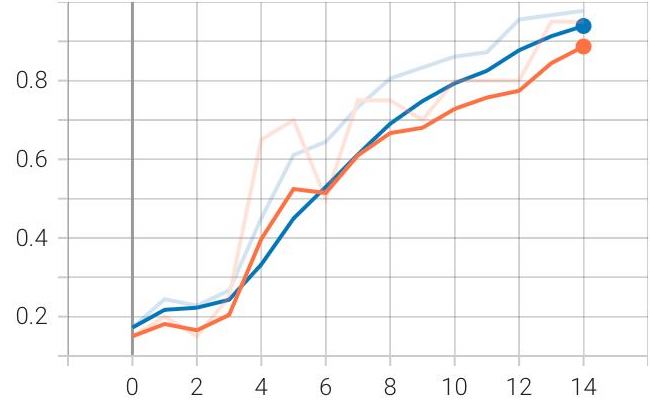
\includegraphics[width=0.7\textwidth]{fig1.jpg}
\caption{\label{fig:fig1} Smoothed model loss over 15 epochs on the training (blue) and validation data (orange), with 0.068 and 0.896, respectively.}
\end{figure}

\noindent
During the training procedure, the performance of our network was tracked by using the tensorboard feature. Figure 1 shows the updated loss over time per epoch, with a loss of 0.068 on the training data after 15 epochs. While loss minimization of the training dataset is a good indicator for model performance, it is still prone to overfitting. Therefore, the class prediction of novel unseen images was tested on the validation dataset, resulting in a loss of 0.896 on the validation data after 15 epochs. We observed a slight increase of the loss after 13 epochs. However, an increasing loss on the validation data after a few epochs does not correlate with the accuracy, as this is the measurement of the final classification decision. Figure 2 shows the prediction accuracy that our model is able to achieve on the data at hand. After 15 epochs, the model was able to predict the image classes of the training data with 97.8\% accuracy, and with an accuracy of 95.0\% on the validation data. In 15 epochs, training the network with the full training dataset and validating the predictions on unseen data took about 21.7 iterations per second and about 2 minutes in total. These results indicate that the model is capable of encoding eye-swiped messages that a dreamer sends to another person in reality.
\\

\begin{figure}[H]
\centering
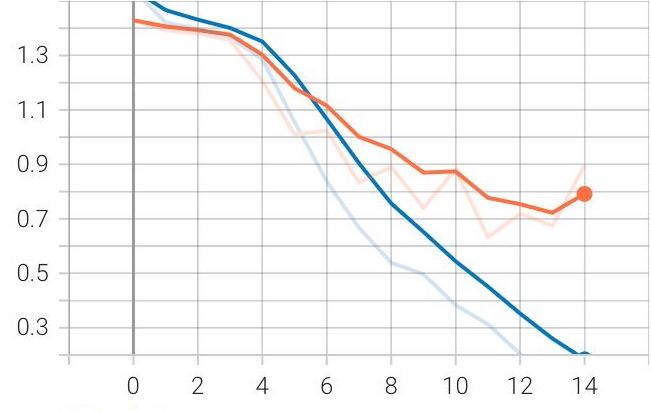
\includegraphics[width=0.7\textwidth]{fig2.jpg}
\caption{\label{fig:fig2} Smoothed prediction accuracy for image classes over 15 epochs on the training (blue) and validation data (orange), with 97.8\% and 95.0\%, respectively.}
\end{figure}



\section{Discussion (Task F)}

In this work, we aimed to train a CNN with dream-related words to enable an eye-swiped message encoded communication for interactive dreaming. A high prediction accuracy on the validation data of 95.0\% was achieved, yielding promising results for future research on interactive dreaming. In combination with more reliable lucid dream induction techniques, the ability to consciously draw eye-swiped messages within a lucid dream might increase, further advancing interactive dreaming and dream research in general. This technique also increases the level of insight into the emotions and experiences of the dream world. Eye-swiped messages have great potential to enable access to dream communication. By training a CNN model on an emotion dataset, we here provide first evidence for an algorithm that can classify messages sent by a dreamer to another person in reality to convey their emotional state while dreaming. The performance of the model suggests that CNN models are suitable for interpretation of such messages during REM sleep.

\subsection*{Potential applications}

Eye-swiped message encoded dream communication could be useful for several reasons. The realization of this form of communication would be a major step in better dream research, as instead of asking participants about their dreams after they wake up in form of dream reports, which is often prone to forgetting the dreamed experience, it would allow for real-time questioning of the dreaming person, which can provide more insight into the person's dream as well as a direct way of guiding the dream in a certain direction. This could influence the dream content and thus open up new possibilities such as acquiring knowledge, therapeutic approaches, or make dreams more entertaining and enjoyable \citep{appel2022sd}. A more futuristic approach like creating art with the recording of eye movements during the dream was mentioned by \citet{appel2022sd}. Another application could be the automatic encoding and forwarding of eye-swiped text messages on text messenger apps to communicate with other people while being inside a dream. Potentially one day, one dreaming person might be able to communicate with another dreaming person with the use of this technique. Also, use cases for the communication with coma patients might be feasible in the future.

\subsection*{Limitations}

Several limitations should be considered while reviewing this paper. Even though the results of the presented CNN seem promising, the technique to record the written words is not even available yet. Additionally, it is not clear if a person while in a lucid dream is even able to draw more complex shapes like words with their eyes since until now, only LRLR eye movements were used to communicate with the waking world in previous research \citep{konkoly2021real}. Also, before being able to respond to questions or report the current emotional state with written words within a dream, one has to reach the state of lucidity. Since the state of art of lucid dream induction techniques are not very reliable \citep[e.g.,][]{saunders2016lucid, stumbrys2012induction}, this form of communication will be very limited to those who are able to become lucid. Because of this problem, upcoming research in this area will be limited. Furthermore, the amount of communication will be limited as well since in our work, only 7 specific words could be encoded. Also, certain tasks like counting or doing sports take longer in a lucid dream than in reality \citep{erlacher2014time}. Therefore, dreaming persons might only be able to write only one word in their short span of lucidity.
\\
This form of real-time communication might transcend the problem that dreamed experiences are often partially forgotten and active dream scenes can be communicated by the dreaming person. Nevertheless, it is very limited, as it is restricted to very short single words and does not allow for an accurate description of the dream or a long answer to the scientists' questions. Therefore, dream reports are crucial as an additional type of questioning for more precise descriptions of the dream content and emotions. 
\\
Furthermore, ethical questions are raised in these regards. First of all, the results of a CNN have to be taken into account with care. Classification errors might lead to misinterpretations of messages from the dreamer, reaching from minor to major consequences, depending on the application. In our case, the dreamer might be woken up after indicating a fearful dream state even though the dream was actually a good one. Moreover, answers to questions during the dream that are misclassified as a “yes” instead of a “no” and vice versa, might be misleading for interpretation of dream content.
\\
Another problem that has to be considered is that, just like for every data-based method, big data approaches may motivate big tech companies to create data profiles about the dream lives of people for personalized advertisement based on dream content.

\subsection*{Conclusion}

Communication between dreamers and wake persons may change the way we do research and open up a variety of useful applications. Here we implemented a CNN that is able to recognize the words “yes” and “no" for basic communication, and classify handwritten emotion-words into their corresponding classes “fear”, “anger”, “disgust”, “happy” and “sad”. We therefore showed that CNNs provide first promising results for application in encoding eye-swiped messages from dreamers. Still, further research for more robust methods, also taking ethical concerns into account is needed to avoid misinterpretation of messages.



% bibtex
%\bibliographystyle{plainnat}
%\bibliography{references}

% biblatex
\printbibliography[title={Bibliography}]
\end{document}
